% !TeX root = ../main.tex
% Add the above to each chapter to make compiling the PDF easier in some editors.

\chapter{The Ray Tracing Approach}\label{chapter:the_raytracing_approach}
In Chapter~\ref{chapter:background} the theoretical background for time-reversal imaging and the utilization of ray tracing for the needed wave-simulation were laid out.
This chapter will describe the implementation of a ray tracing approach for the time-reversal imaging algorithm.

As mentioned in \parencite{dyab_critical_2013} the quality of the time-reversed image increases within a highly reverberant environment.
In contrast to other imaging algorithms, multipath propagation of the waves is therefore not suppressed but used to improve the time-reversal imaging.
To simulate the multipath propagation, one is interested in all the paths that the signal takes from the source to the imaging domain.
The multipath propagation is mostly caused by reflections and refractions which can be described by the laws of geometrical optics as shown in Section~\ref{sec:ray-concept}.
This is why ray tracing is such a suitable approach for this problem.

\section{The Imaging Algorithm}
The time-reversal imaging algorithm is a three-step process.
First, the scene is illuminated with a monochromatic signal of frequency \(\omega_i\) and the resulting scattered field is recorded at \(M\) receiver locations \(\bm{r}_j\). 
This step is repeated for \(N\) frequencies \(\omega_i\) resulting in the \(N \times M\) matrix \(\mathsf{E} \) containing the scattered field at all receiver locations for all frequencies.

In the second step, a random location in the target domain is chosen as the source of a big number of rays (\(N_{\text{rays}}\approx 10^{9}\)) which are launched into equally distributed random directions.
A ray that follows a possible path from the target location to a receiver location will eventually hit the receiver so the path can be recorded.
From these paths, the paths for the other locations in the target domain can be derived by using virtual targets as described in Section~\ref{section:virtual_targets}.
This step is necessary because shooting \(N_{\text{rays}}\) rays in all directions from all points in the target domain would be computationally expensive.

The virtual targets resulting from the second step are then grouped into wavefronts, which are further described in Section~\ref{section:subdivision_into_wavefronts}.
Finally, the field contribution of each wavefront at any point in the imaging domain is calculated.
The measured scattered field \(\underline{\mathsf{E}}\) is complex conjugated and sent back from every corresponding receiver to all points in the imaging domain along the paths of this wavefront.
The calculation of the field propagation along this ray-path from one hit-point to the next is described in Section~\ref{section:calculation_of_the_field_propagation}.

The sum of all receiver contributions at each point in the imaging domain then gives rise to the time-reversed field of this wavefront in the imaging domain.
By taking the absolute value of the time-reversed field, the image is obtained.
For a better resolution of the image, this step is repeated for all measured frequencies \(\omega_i\).
This can be summarized in the imaging formula of the n-th wavefront
\begin{equation}
    I_n(\bm{r}_k) = |\sum_{i=1}^{N} \sum_{j=1}^{M} \underline{\mathsf{E}}_{ij}^* \cdot H_{j \rightarrow k}(\omega_i)|
\end{equation}
where \(H_{j \rightarrow k}(\omega_i)\) is the transfer function from receiver \(j\) to point \(k\) in the imaging domain at frequency \(\omega_i\) along the n-th wavefront, which is calculated by tracing the electric field along the ray-path according to~\eqref{eq:field-along-ray-path}.


\section{Implementation of Virtual Targets for Multipath Wave Propagation}\label{section:virtual_targets}

\begin{figure}[ht]
    \centering
    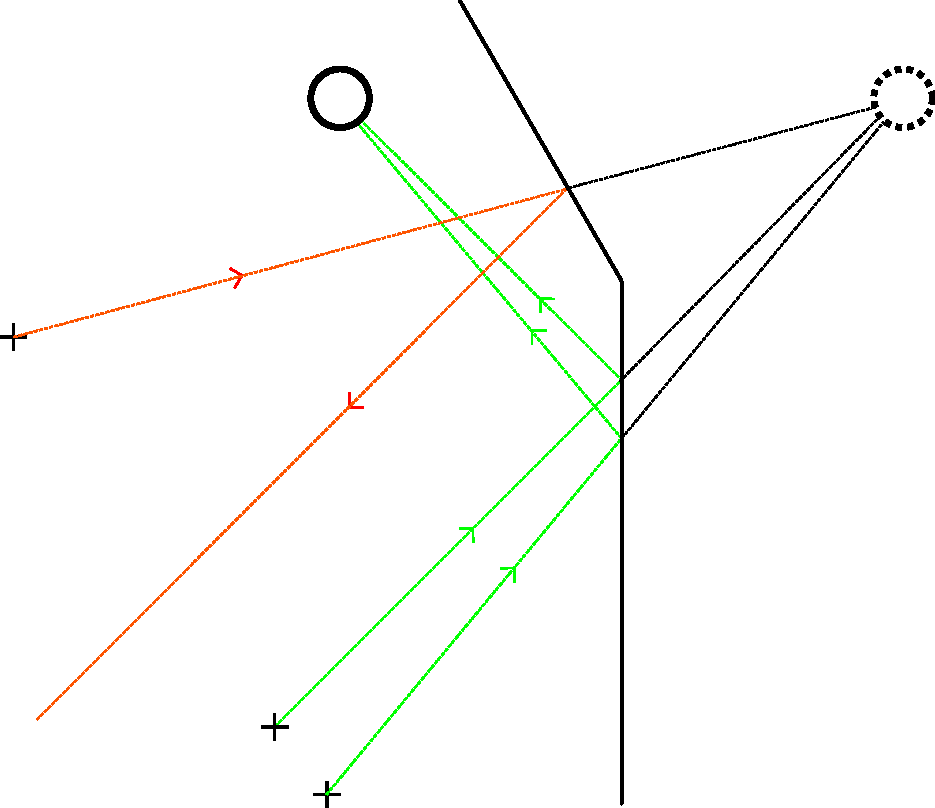
\includegraphics[width=0.5\textwidth]{build/VirtualTargets.pdf}
    \caption{The green paths show, how shooting a ray at a virtual target (dotted circle) from different locations can result in hitting the original target (full line circle). The red path on the other hand does not hit the target because its launch location is too far away from the other launch locations.}\label{fig:virtual_targets}
\end{figure}

To derive the paths for all points in the imaging domain from the paths of a single point in the imaging domain, the concept of virtual targets is used.
In the following, the initial single point in the imaging domain is called the probe point.

A path is distinguished by its launch location, the receiver where it ends, and the sequence of plane surfaces it encounters between the launch point and the receiver.
The receiver is modelled as a sphere with radius \(r_{\text{rec}}\) around the receiver location.
This radius should be chosen big enough, so the randomly generated rays do not all miss the receiver, but small enough to not overlap with other receivers.
If a ray launched from the probe point \(\bm{r}_p\) with the initial direction \(\bm{u}_{\text{init}}\) hits a receiver, any point \(\bm{p} = \bm{r}_p + s \cdot \bm{u}_{\text{init}}\) can be used to reconstruct the path between the probe point and the receiver in the following time-reversal step.
To do this one simply has to shoot a ray from the probe point in the direction of \(\bm{p}\).

\begin{figure}
    \centering
    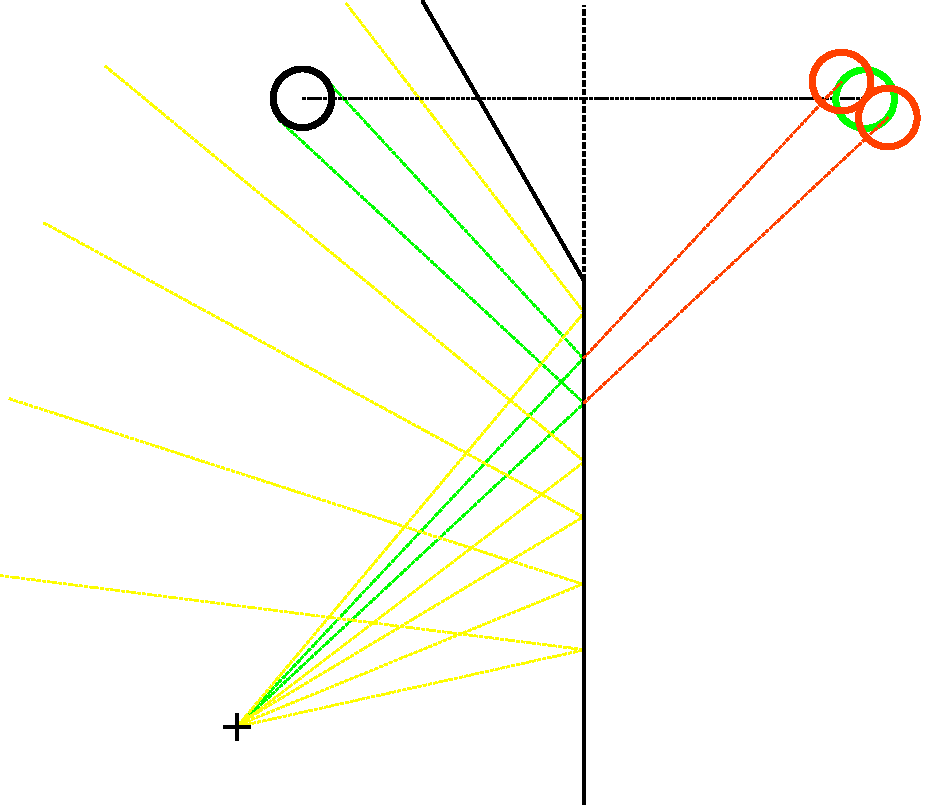
\includegraphics[width=0.5\textwidth]{build/VirtualTargetsMultiHit.pdf}
    \caption{Two random rays hit the receiver sphere, so two virtual targets would be created (red circles) although there should be only one virtual target (green circle) at the mirrored position of the receiver circle.}\label{fig:mulithit}
\end{figure}

Setting \(s\) to the distance \(d\) that the ray traveled results in the corresponding virtual target \(\bm{v}\).
\begin{equation}\label{eq:visual_target}
    \bm{v} = \bm{r}_p + d \cdot \bm{u}_{\text{init}}
\end{equation}
Shooting a ray from any point \(\bm{r}_k\) close to the probe point in the direction of the virtual target will in most cases hit the same receiver, so the virtual target can be used to reconstruct the path between \(\bm{r}_k\) and the receiver as well  (see Figure~\ref{fig:virtual_targets}).

It is important to stress that this approach only works for points close to the probe point.
If the point is too far away, a ray shot at the virtual target might not hit the receiver.
In a similar way, the virtual targets found for the probe point might not account for all the paths between an imaging point and the receiver.

Another problem arises with this approach when multiple rays with slightly different launch directions hit the same receiver taking the same path (see Figure~\ref{fig:mulithit}).
In this case two virtual targets would be recorded for one actual path.
This would lead to an unwanted increased influence of this path in the time-reversal step.
To resolve this issue, every ray has an associated hash value that is calculated from the path it takes, i.e.~from the object-ID's of the plane surfaces it bounces of and the receiver it finally hits.
This way it can be checked if a virtual target for this path has already been recorded, as every path has an unique hash value.
If this is the case, the new virtual target is not saved.

Furthermore, equation~\eqref{eq:visual_target} is only an approximation of a perfect virtual target, which would be retrieved by mirroring the receiver location at the plane surfaces the ray hits in a backwards manner.
For the sake of simplicity, this is not done in the implementation.
Instead the center of the hit sphere \(\bm{r}_{\text{receiver}}\) is projected on the linear slope of the ray to retrieve a more accurate value for the distance between launch location and receiver along the path.

\begin{equation}
    d_{\text{approx}} = d_{\text{ray\_hit}} +  (\bm{r}_{\text{receiver}} - \bm{r}_{\text{ray\_hit}}) \cdot \bm{u}_{\text{ray\_hit}} \approx d_{\text{actual}}
\end{equation}

\begin{figure}[h]
    \centering
    \def\svgwidth{0.5\textwidth}
    \input{build/d_approx.pdf_tex}
    \caption{Projection of \(\bm{r}_{\text{receiver}}\)}\label{fig:d_approx}
\end{figure}
 

\section{Subdivision Into Wavefronts}\label{section:subdivision_into_wavefronts}
Every virtual target recorded in the preceding step is a version of one of the receivers that was mirrored at the plane surfaces the ray hit.
By shooting rays at them from the imaging domain, the paths between the imaging domain and the receiver locations are reconstructed and therefore the according transfer functions can be simulated.
A subset of virtual targets which accounts for one mirrored version of all receiver locations is called a wavefront.
There are as many wavefronts as there are different paths from one receiver to the probe point.
The virtual targets are mapped to the wavefronts by the hash value of the ray before including the hit receivers object-ID into the hash calculation.
This way, the wavefronts are characterized by the sequence of plane surfaces the rays reflect of.

The term wavefront is used because the paths of the rays to the virtual targets of one wavefront can be seen as the paths of a common wavefront that is emitted from the receiver location.
The subdivision of the virtual targets into wavefronts is done to get more insight into the imaging contribution of each wavefront.
To retrieve the final time-reversed image, the images of all wavefronts simply have to be summed up.


\section{Calculation of the Field Propagation}\label{section:calculation_of_the_field_propagation}
As shown in Equation~\eqref{eq:field-along-ray-path}, the propagation of the electric field along the ray-path according to the path-length \(l\) is calculated by:
\begin{equation}
    \underline{E}(l) = \frac{1}{1 + l} \cdot \underline{E}_0 \cdot \mathrm{e}^{\mathrm{i} k_0 \cdot n \cdot l}
\end{equation} 

The ray tracing program will calculate the location where a ray hits a plane surface (or receiver sphere respectively) and the direction of the reflected ray.
To efficiently trace the field along the ray-path, the resulting field \(\underline{E}_{\text{new}}\) at the hit location should be calculated from the field \(\underline{E}_{\text{old}}\) at the previous hit location (or the launch location respectively), the length of the path at this old hit location \(l_{\text{old}}\) and the distance \(d\) between the old and the new hit point.
\begin{equation}
    \underline{E}_{\text{new}} = \underline{E}_{\text{new}}(l_{\text{new}}) = \underline{E}_{\text{new}}(\underline{E}_{\text{old}}, l_{\text{old}}, d)
\end{equation}
Considering that \(l_{\text{new}} = l_{\text{old}} + d\) the new field can be written as
\begin{equation}
    \underline{E}_{\text{new}} = \frac{1}{1 + l_{\text{old}} + d} \cdot \mathrm{e}^{\mathrm{i} k_0 \cdot n \cdot d}  \cdot \underline{E}_{0} \cdot \mathrm{e}^{\mathrm{i} k_0 \cdot n \cdot l_{\text{old}}} 
\end{equation}
With \(\underline{E}_{\text{old}} = \frac{1}{1 + l_{\text{old}}} \cdot \underline{E}_0 \cdot \mathrm{e}^{\mathrm{i} k_0 \cdot n \cdot l_{\text{old}}} \) the formula for \(\underline{E}_{\text{new}}(\underline{E}_{\text{old}}, l_{\text{old}}, d)\) is retrieved:
\begin{equation}
    \underline{E}_{\text{new}}(\underline{E}_{\text{old}}, l_{\text{old}}, d) = \underline{E}_{\text{old}} \cdot \frac{1 + l_{\text{old}}}{1 + l_{\text{old}} + d} \cdot \mathrm{e}^{\mathrm{i} k_0 \cdot n \cdot d}
\end{equation}
